% % % % % % % % % % % % % % % % % % % % % % % % % % % % % % % % % % % % % % % % %
\section{Freie Theoreme}
% % % % % % % % % % % % % % % % % % % % % % % % % % % % % % % % % % % % % % % % %

\label{sec:freie-theoreme}

Betrachtet man eine Typsignatur in Haskell, dann hat man intuitiv eine Vorstellung davon, was diese Funktion ungefähr
macht. Je nach Typ kann die Funktion in ihrer Funktionsweise stark eingeschränkt sein, was Haskells Typsystem zu verdanken
ist, genauer: dem parametrischen Polymorphismus. Nicht nur verringert dieses Typsystem die Fehleranfälligkeit von
produziertem Code, es vereinfacht auch Rückschlüsse auf die Funktionsweise und Korrektheitsbeweise.

Wie in der Einleitung bereits angedeutet wurde, lässt sich diese Intuition in Formeln ausdrücken. In diesem Abschnitt
wird erklärt, wie diese so genannten freien Theoreme aussehen. Es wird erläutert, wie man sie herleitet und warum
das möglich ist. Am Ende des Abschnittes wird insbesondere darauf eingegangen, welche Rolle Typkonstruktorklassen
für die Generierung von freien Theoremen spielen.

%Einleitend wurde bereits das mächtige Typsystem Haskells angesprochen. Dieses Typsystem ist komplett statisch und
%unterstützt parametrischen Polymorphismus, wie in den Grundlagen erläutert wurde. Nicht nur verringert ein solches Typsystem
%die Fehleranfälligkeit von produziertem Code, es vereinfacht auch Rückschlüsse auf die Funktionsweise und Korrektheitsbeweise.
%In dieser Arbeit geht es vor allem um die bereits angesprochenen freien Theoreme. Diese lassen sich herleiten, ohne dass man
%überhaupt die konkrete Implementierung in Betracht ziehen muss. Man nennt sie ``freie Theoreme'', weil man sie gewissermaßen
%``geschenkt'' bekommt. Wie genau man diese Theoreme herleitet, soll in diesem Abschnitt genauer erläutert werden.


% - - - - - - - - - - - - - - - - - - - - - - - - - - - - - - - - - - - - - - - - - - - - - - - - - - - - - - - - - - - - - - - - - - - - - - - - - - - - - -
\subsection{Beispiel}
% - - - - - - - - - - - - - - - - - - - - - - - - - - - - - - - - - - - - - - - - - - - - - - - - - - - - - - - - - - - - - - - - - - - - - - - - - - - - - -

Bevor die theoretische Herangehensweise beschrieben wird, bietet es sich zunächst an, die Vorgehensweise an einem Beispiel
intuitiv zu erklären. Erst danach wird das Vorgehen konkretisiert und in Formeln dargestellt.
Als Beispiel soll die folgende Haskell-Typsignatur dienen.
%Zunächst bietet es sich an, die Vorgehensweise an einem konkreten Beispiel vorzuführen. Bevor es um die theoretische
%Herangehensweise geht, soll das Vorgehen erst einmal intuitiv motiviert werden. Wir betrachten die folgende Haskell-Funktion.

\begin{align*}
f :: [a] \rightarrow [a]
\end{align*}

Gegeben ist also eine Funktion $f$, die von einer Liste auf eine Liste abbildet. Das Besondere an dieser Funktion ist, dass sie
nicht für einen konkreten Typ wie beispielsweise $[Integer] \rightarrow [Integer]$ definiert ist, sondern dass man sie für jeden
beliebigen Typsignatur instanziieren kann, indem man für die Typvariable $a$ einen Typausdruck einsetzt. Es handelt sich
um eine \textit{polymorphe Funktion}. Instanziierung einer polymorphen Funktion auf einen bestimmten Typ wird im Folgenden
durch eine Index-Schreibweise dargestellt. $f_{Integer}$ wäre also eine Funktion mit dem Typen $[Integer] \rightarrow [Integer]$,
$f_{Bool}$ wäre die gleiche Funktion für den Typen $[Bool] \rightarrow [Bool]$.
%3sie für jeden beliebigen Typen,
%der für die Typvariable a eingesetzt werden
%kann. Es handelt sich also um eine polymorphe Funktion.

Bei Polymorphismus ist zwischen Ad-Hoc Polymorphismus und parametrischem Poly\-mor\-phis\-mus zu unterscheiden. Typvariablen
in Haskell entsprechen dem parametrischen Polymorphismus, das heißt die entsprechende Funktion arbeitet für sämtliche
eingesetzten Typen nach demselben Prinzip.
%In diesem Fall handelt es sich um parametrischen Polymorphismus, d.h. die Funktion arbeitet für sämtliche Typen nach dem gleichen Prinzip.

Das ist deswegen etwas Besonderes, weil es dadurch ermöglicht wird, allgemeine Aussagen zu treffen, die für sämtliche
Typinstanziierungen gelten. Vergleicht man diese Methode mit Ad-Hoc-Polymorphismus, wird der Vorteil klar: Unter Letzterem
versteht man, dass eine Funktion zwar für verschiedene Typen definiert wird, diese jedoch jeweils eine konkrete,
typspezifische Implementierung haben.

Es handelt sich also eigentlich um verschiedene Funktionen, die sich einen Namen teilen, weil anhand der Typen entschieden
werden kann, welche der Funktionen jeweils angewandt werden muss.
Diese Implementierungen können also komplett unterschiedlich funktionieren und kennen den konkreten Typen, für den sie
implementiert sind, können also auf typspezifische Eigenschaften zugreifen. Man kann sich denken, dass das allgemeine Aussagen
unmöglich macht.

Die vorliegende Funktion des Beispiels ist also für jeden beliebigen Typ $a$ definiert. Das hat Konsequenzen für
deren Funktionsweise. Man kann sich an dieser Stelle die Frage stellen: Wie kann die
Funktion die Ergebnisliste erzeugen? Sie kennt den konkreten Typ nicht, das heißt sie kann keine neuen Elemente ``erfinden''.
Eine Möglichkeit hat sie aber dennoch: Sie kann die Elemente der Eingabeliste wiederverwenden.
%sie kann lediglich auf die Elemente der Eingabeliste zurückgreifen. Die
Die einzige Möglichkeit für die Funktion, die Liste zu ändern, besteht also in einer Umsortierung der Listenelemente.

Doch auch für eine Neusortierung der Liste hat die Funktion wenig Anhaltspunkte. Sie kennt zwar die Länge der Liste, doch ohne Kenntnis des Typen kann sie keine weiteren Aussagen über den Inhalt der einzelnen Listenelemente treffen (und da die Klasse Eq
nicht gegeben ist, nicht mal über deren Gleichheit).
Sie wird also gezwungenermaßen je zwei Listen gleicher Länge stets gleich behandeln.
%Sie wird also für zwei Listen gleicher Länge $l$ und $l'$ exakt das Gleiche tun.

Bevor weiter argumentiert werden kann, soll an dieser Stelle eine bekannte Funktion aus Haskell eingeführt werden. Die Funktion
\texttt{$map :: (a \rightarrow b) \rightarrow [a] \rightarrow [b]$} erwartet eine Funktion als ersten Parameter und eine Liste als
zweiten Parameter. Sie erzeugt aus der Liste eine neue gleicher Länge, indem jedes Element mit der übergebenen Funktion in
ein neues Element überführt wird.

Haskell verwendet für Funktionsapplikation das Prinzip des Currying, das heißt, dass eine Funktion mit $n$ Parametern, die auf ein
Argument angewandt wird, eine neue Funktion zurückgibt, die noch $n-1$ Parameter erwartet. \todo{quote} Man kann die
die $map$-Funktion also auch anders interpretieren: $map$, angewandt auf eine Funktion, gibt eine Funktion zurück, die
die Funktionalität der Eingabefunktion für Listen bietet, sie also in den Listen-Kontext \textit{liftet}.
%Da Haskells Funktionsapplikation das Prinzip des Currying verwendet, \todo{quote?} kann man diese Funktion auch auf eine andere
%Weise interpretieren: $map$, angewandt auf eine Funktion, \textit{liftet} diese in den Listen-Kontext, gibt also eine Funktion zurück,
%die dieselbe Funktionalität für Listen bietet.

Wir betrachten jetzt eine beliebige nicht-polymorphe Funktion $g$, die auf dem konkreten Typ arbeitet, auf den die
Beispielfunktion $f$ instanziiert wurde. $map\ g$ liefert folglich eine Funktion, die $g$ auf sämtliche Elemente einer Eingabeliste
anwendet. Jede Liste, die durch Anwendung von $map\ g$ entsteht, wird die gleiche Anzahl an Elementen haben wie vorher.
Darüber hinaus vertauscht $map\ g$ die Listenelemente nicht, jedes neue Element wird an derselben Stelle stehen wie
sein Ursprungselement.

Auf dieser Argumentation aufbauend kann man erkennen, dass es unerheblich für die Ergebnisliste ist, ob man zuerst die
Funktion $f$ auf eine Liste appliziert und dann auf die resultierende Liste die Funktion $map\ g$ anwendet, oder ob man
in umgekehrter Reihenfolge vorgeht. Die folgende Formel fasst diese Aussage mathematisch zusammen.


%Die Haskell-Funktion \texttt{$map :: (a \rightarrow b) \rightarrow [a] \rightarrow [b]$} wendet eine Funktion auf jedes Element einer Liste an und gibt die resultierende Liste zurück. Da Haskell Currying für Funktionsapplikation verwendet, kann man
%diese Funktion auch auf eine andere Weise interpretieren: $map$, angewandt auf eine Funktion, liftet diese in den Listen-Kontext,
%gibt also eine Funktion zurück, die dieselbe Funktionalität für Listen bietet. Betrachten wir nun eine beliebige Funktion $g :: a \rightarrow a$. Es lassen sich jetzt Aussagen über $map\ g$, angewandt auf Listen, treffen. Zum einen wird jede Liste, auf die man $map\ g$ anwendet, die gleiche Länge haben wie vorher - das liegt einfach in der Natur von $map$.

%Darüber hinaus müssen jeweils zwei Elemente, die an der gleichen Position stehen, auf die gleiche Weise entstanden sein, nämlich
%durch Anwenden von $g$ auf das entsprechende Listenelement.
%Es ist nun logisch, dass es egal ist, ob man zuerst die Funktion f auf eine Liste anwendet und dann die Funktion g auf die
%resultierende Liste mappt, oder ob man in umgekehrter Reihenfolge vorgeht.

\begin{align*}
f (map\ g\ l) = map\ g\ (f\ l)
\end{align*}

Diese Aussage ist ein Theorem, das für beliebige Funktionen g und beliebige Listen l gilt. Doch nicht nur das: Wir haben für
die Herleitung kein Wissen über die konkrete Implementierung der Funktion f benötigt; das einzig Bekannte war die Typsignatur.
Das Theorem gilt also insbesondere für alle Funktionen mit der Typsignatur $[a] \rightarrow [a]$. Da man dieses Theorem
aus der Typsignatur ``geschenkt'' bekommt, wird es auch ``freies Theorem'' genannt.
Natürlich war die vorangegangene Herleitung sehr unkonkret und nicht wirklich mathematischer Natur. Daher soll im Folgenden
erklärt werden, wie man freie Theoreme im Allgemeinen und vor allem auf mathematischer Grundlage herleitet.


% - - - - - - - - - - - - - - - - - - - - - - - - - - - - - - - - - - - - - - - - - - - - - - - - - - - - - - - - - - - - - - - - - - - - - - - - - - - - - -
\subsection{Parametrizität}
% - - - - - - - - - - - - - - - - - - - - - - - - - - - - - - - - - - - - - - - - - - - - - - - - - - - - - - - - - - - - - - - - - - - - - - - - - - - - - -

\label{sec:free-theorems-param}

Der Schlüssel zur Herleitung von freien Theoremen liegt in der Betrachtung von Typen.
Intuitiv werden Typen gerne als Mengen aufgefasst. So würde man den Typen \texttt{Bool} beispielsweise als Menge $\mathbb{B}$
der booleschen Werte auffassen mit $\mathbb{B} = \{ tt, ff \}$, der Typ \texttt{Integer} wäre die Menge der ganzen Zahlen
$\mathbb{Z}$ usw. Komplexere Typen ergeben sich dann durch Zusammensetzung aus einzelnen Basistypen, beispielsweise
würde man den Typen \texttt{$Integer \rightarrow Integer$} auffassen als die Menge $(\mathbb{Z} \rightarrow \mathbb{Z})$ aller Funktionen von den ganzen Zahlen in die ganzen Zahlen.

Die grundsätzliche Idee hinter freien Theoremen basiert auf der Erkenntnis von Reynolds, dass die Semantik eines beliebigen
Ausdrucks verwandte Umgebungen auf verwandte Werte abbildet \cite{reynolds}. Dieses Theorem, von Reynolds das
\textit{Abstraktionstheorem} genannt, wird von Wadler umformuliert zum sogenannten \textit{Parametrizitätstheorem} \cite{wadler},
das im Folgenden erläutert werden soll. Entscheidend ist, dass man Typen nicht als Mengen sondern als Relationen ausdrückt,
um dieses Theorem anwenden zu können.

%Für die Herleitung von freien Theoremen ist diese Repräsentation nicht ganz ausreichend, da sie spätestens bei polymorphen
%Typen auf beweistechnische Probleme stößt \todo{?}. Daher greift man auf eine etwas andere Repräsentation zurück: Man
%betrachtet Typen als Relationen.

%Man kann zu einem Typen nun systematisch eine Relation konstruieren, die diesen Typen repräsentiert. Dazu geht man
%folgendermaßen vor:

Man kann zu einem beliebigen Typ eine Relation konstruieren, die diesen Typ repräsentiert. Dazu geht man folgendermaßen vor.

\begin{itemize}
\item Zu jedem Basistyp $T$ (Int, Bool, etc.) ist die zugehörige Relation die Identitätsrelation $\mathcal{R} = \{ (x, x) | x \in T\}$.
\item Sind $\mathcal{R} : R_1 \Leftrightarrow R_2$ und $\mathcal{S} : S_1 \Leftrightarrow S_2$ Typrelationen, so ist $\mathcal{R} \rightarrow \mathcal{S} = \{ (f, g) | f \in (R_1 \rightarrow R_2), g \in (S_1 \rightarrow S_2), \forall x \in R_1, y \in R_2: (f\ x, g\ y) \in \mathcal{S} \}$ die zugehörige Funktionstyprelation.
\item Ist $\mathcal{F}(\mathcal{X})$ eine Typrelation, die von einer Typrelation $\mathcal{X}$ abhängt, dann definiert man
$\forall \mathcal{X} . \mathcal{F}(\mathcal{X}) = \{ (x, y) | \forall A_1, A_2 \in Typen, \mathcal{A} : A_1 \Leftrightarrow A_2: 
(x_{A_1}, y_{A_2}) \in \mathcal{F}(\mathcal{A}) \}$. Hierbei sind $x$ und $y$ polymorphe Elemente, die durch $x_{A_1}$ und
$y_{A_2}$ auf einen bestimmten Typ instanziiert werden.
\end{itemize}

Zudem lassen sich bestimmte Typkonstruktoren, wie beispielsweise der Listenkonstruktor $[a]$, durch Lifting der betreffenden
Relation umsetzen. Man kann beispielsweise für eine gegebene Typrelation $\mathcal{R} : T_1 \Leftrightarrow T_2$ folgenes
Lifting definieren.

\begin{align}
[\mathcal{R}] = \{ ([], []) \} \cup \{ (a : as, b : bs) | (a, b) \in \mathcal{R}, (as, bs) \in [\mathcal{R}] \}
\end{align}

Andere Standardtypkonstruktoren lassen sich auf ähnliche Weise beschreiben. Nun haben wir die Mittel, zu jeder vorhandenen
Typsignatur eine Relation zu konstruieren. Eine entscheidende Erkenntnis von \cite{wadler}, aufbauend auf
\cite{reynolds}, ist nun folgende: Ist t ein geschlossener Term von Typ T und $\mathcal{T}$ die zugehörige konstruierte
Typrelation, dann gilt $(t, t) \in \mathcal{T}$ (dieser Satz wird von \cite{wadler} auch Parametrizität, \textit{Parametricity}, genannt).

Damit ist alles gegeben, was man zur Herleitung des freine Theorems benötigt. Wir untersuchen wieder das Beispiel
$f :: [a] \rightarrow [a]$. Durch Parametrizität ist gegeben:

\begin{align}
(f, f) \in \forall \mathcal{R} . [\mathcal{R}] \rightarrow [\mathcal{R}]
\end{align}

Dabei ist zu bemerken, dass in Haskellsyntax typischerweise die Allquantifizierung über die Typvariable weggelassen wird.
Implizit ist $[a] \rightarrow [a]$ aber gleichbedeutend mit $\forall a . [a] \rightarrow [a]$.
Wir können nun Schritt für Schritt die Definitionen der einzelnen Relationskonstruktionen anwenden, wodurch die Formel
abgerollt wird:

\begin{align*}
&\forall A_1, A_2 \in Typen, \mathcal{A} : A_1 \Leftrightarrow A_2: \\
&(f_{A_1}, f_{A_2}) \in [\mathcal{A}] \rightarrow [\mathcal{A}] \\
& \\
\Leftrightarrow &
\forall A_1, A_2 \in Typen, \mathcal{A} : A_1 \Leftrightarrow A_2: \\
& \forall (l, l') \in [\mathcal{A}]: \\
&(f_{A_1} l, f_{A_2} l') \in [\mathcal{A}] \\
& \\
\Leftrightarrow &
\forall A_1, A_2 \in Typen, \mathcal{A} : A_1 \Leftrightarrow A_2: \\
& \forall (l, l') \in lift_{[]}(\mathcal{A}): \\
& (f_{A_1} l, f_{A_2} l') \in lift_{[]}(\mathcal{A}) \\
\end{align*}

Zur Erinnerung: $\mathcal{A} : A_1 \Leftrightarrow A_2$ bedeutet, dass $\mathcal{A}$ eine Relation auf den Mengen $A_1$ und $A_2$ ist.

An diesem Punkt haben wir eine Aussage über beliebige Typrelationen $\mathcal{A}$, anschaulicher wäre aber eine Aussage
über beliebige Funktionen. Da man Funtktionen als Spezialfall von Relationen betrachten kann, können wir die Aussage
spezifizieren für den Fall, dass es sich bei $\mathcal{A}$ um eine Funktion handelt.
Eine Funktion $f : S \rightarrow T$ kann man auch betrachten als Relation $\{ (x, f x) | x \in S \}$. Anders gesagt: Ist
$\mathcal{F} : T_1 \Leftrightarrow T_2$ eine Relation zu einer Funktion f, dann gilt für alle $(x, y) \in \mathcal{F}: f x = y$.

Schränken wir also unsere Aussage auf Funktionen ein, können wir über alle Funktionen $g : A_1 \rightarrow A_2$ quantifizieren.
Wir wissen, dass für alle Parameter $l, l' \in lift_{[]}(\mathcal{A})$ die Aussage $(f_{A_1} l, f_{A_2} l') \in lift_{[]}(\mathcal{A})$
gilt. Als Funktion geschrieben heißt das, es gilt:

\begin{align}
lift_{[]}(g) (f_{A_1}\ l) = f_{A_2}\ l'
\end{align}

Das Lifting von Funktionen in den Listenkontext ist ganz einfach das Mapping dieser Funktion auf Listen, sprich: die Haskell-Funktion
$map$, angewandt auf die entsprechende Funktion:

\begin{align}
map\ g\ (f_{A_1}\ l) = f_{A_2}\ l'
\end{align}

Da $(l, l') \in [A]$, können wir $l'$ auch anders ausdrücken als $map\ g\ l = l'$. Man erhält also:

\begin{align}
map\ g\ (f_{A_1} l) = f_{A_2} (map\ g\ l)
\end{align}

Und man erkennt: Es handelt sich um die gleiche Aussage, die wir vorher intuitiv konstruiert haben. Jetzt haben wir bewiesen,
dass sie gültig ist, da Parametrizität gilt. Und ein Theorem dieser Art lässt sich für jede beliebige Typsignatur herleiten.


% - - - - - - - - - - - - - - - - - - - - - - - - - - - - - - - - - - - - - - - - - - - - - - - - - - - - - - - - - - - - - - - - - - - - - - - - - - - - - -
\subsection{Typkonstruktorklassen und -variablen}
% - - - - - - - - - - - - - - - - - - - - - - - - - - - - - - - - - - - - - - - - - - - - - - - - - - - - - - - - - - - - - - - - - - - - - - - - - - - - - -

\label{sec:typkonstruktorklassen}

Eine Sache, die bisher nur kurz angerissen wurde, ist die relationale Interpretation von Typkonstruktoren.
Für den Listentypkonstruktor wurde eine Formel gegeben, mit der eine Relation in den Listenkontext geliftet wird.
Ähnlich kann man auch bei anderen Typen vorgehen, beispielsweise $Maybe$.

Was aber völlig ignoriert wurde ist die Tatsache, dass man in Haskell auch über Typvariablen allquantifizieren kann, die ihrerseits
nicht Platzhalter für speziellele Typen, sondern nur für Typkonstruktoren sind. Hier noch einmal das Beispiel aus der Einleitung:

\begin{minted}{haskell}
fmap :: Functor f => (a -> b) -> f a -> f b
\end{minted}

Es wird angegeben, dass $f$ eine Variable der Typklasse Funktor ist. Functor ist von der \textit{Sorte} $* \rightarrow *$,
das heißt es handelt sich um einen Typkonstruktor, der einen Typ auf einen neuen Typ abbildet.
Daher kann $f$ in der Typsignatur in $f a$ und $f b$ auf Parameter angewandt werden.
Zwei Dinge müssen zum bisherigen Ansatz hinzugefügt werden: Allquantifizierung über Typkonstruktorvariablen muss separat betrachtet werden, und Klasseneinschränkungen müssen beachtet werden, im obigen Beispiel $Functor f$ \cite{voigtlander}.

Die Allquantifizierung über Typkonstruktorvariablen funktioniert an sich ähnlich wie die Allquantifizierung über gewöhnliche
Typvariablen. Statt beliebigen Relationen über beliebig gewählten Typen interpretiert man freie Typkonstruktorvariablen als
Funktionen über Relationen mit beliebig gewählten Typkonstruktoren \cite{voigtlander}.

Dazu kommt noch die Beschränkung auf bestimmte Klassen. In einer Klassendefinition legt man Typparameter sowie
Klassenfunktionen fest. Als Beispiel bietet sich die Klassendefinition von Functor an, hier beschränkt auf die interessante Funktion
$fmap$:

\begin{minted}{haskell}
class Functor f where
  fmap :: (a -> b) -> f a -> f b
\end{minted}

Wie man sieht, hat die Klasse Functor einen Typparameter $f$ und definiert die Typsignatur zu $fmap$. Stößt man jetzt in
einer Typsignatur auf eine Klassenbeschränkung wie $Functor f$ (ohne die Typkonstruktorvariablen wenig Sinn machen),
muss man die Allquantifizierung über Typkonstruktoren weiter einschränken.

Sei $\mathcal{F}(\mathcal{X})$ wieder eine Typrelation, die von Typrelation $\mathcal{X}$ abhängt, und sei C eine Typklasse. Wir definieren Allquantifizierung über Typkonstruktorvariablen als:

\begin{align*}
\forall^{\{C\}} \mathcal{K} . \mathcal{F}(\mathcal{K}) = \{ 
(x_{k1}, x'_{k2}) | k_1, k_2 \text{Typkonstruktoren für C, die C einhalten},\\
\mathcal{A} : k_1 \Leftrightarrow k_2, (x, x') \in \mathcal{F}(\mathcal{A})
\}
\end{align*}

Was ist nun mit Typkonstruktoren gemeint, die die Klasse C \textit{einhalten}? Es werden nur jene Typkonstruktoren in Betracht gezogen,
für die jede Klassenfunktion bezüglich ihrer Typrelation mit sich selbst verwandt ist. Für unser Beispiel bedeutet das, es werden nur
Funktionen $\mathcal{F} : k_1 \Leftrightarrow k_2$ betrachtet, für die gilt:

\begin{align*}
(fmap_{k_1}, fmap_{k_2}) \in \forall \mathcal{R} . (\mathcal{R} \rightarrow \mathcal{S}) \rightarrow \mathcal{F} \mathcal{R}
\rightarrow \mathcal{F} \mathcal{S}
\end{align*}

Die Anwendung von Typkonstruktorfunktionen auf Typrelationen ist nun nichts anderes als wiederum ein Lifting dieser
Relation - mit dem Unterschied, dass wir erstmal keine genauen Aussagen über dieses Lifting treffen können.

%Eine Frage, die sich nun stellt, ist: Inwiefern kann man dann überhaupt mit diesen Relationsfunktionen arbeiten? An sich ist ja nur
%bekannt, dass sie Typrelationen auf andere Typrelationen abbilden. Mit der Klassenbeschränkung ist aber zumindest ein
%Anhaltspunkt gegeben. So kann man im Fall der $Functor$ Klasse beispielsweise davon ausgehen, dass es in irgendeiner
%Art und Weise möglich sein muss, den ``Inhalt'' des Functors zu manipulieren - eine Art ``natürliches'' $map$ 
%\todo{Quelle? Beweis?}, das im folgenden $map_F$ genannt wird.


% - - - - - - - - - - - - - - - - - - - - - - - - - - - - - - - - - - - - - - - - - - - - - - - - - - - - - - - - - - - - - - - - - - - - - - - - - - - - - -
\subsection{Anwendung}
% - - - - - - - - - - - - - - - - - - - - - - - - - - - - - - - - - - - - - - - - - - - - - - - - - - - - - - - - - - - - - - - - - - - - - - - - - - - - - -

In den vorangehenden Abschnitten wurde beschrieben, wie freie Theoreme hergeleitet werden. Um zu zeigen, welchen
Nutzen diese Technik hat und was man damit herleiten kann, werden in diesem Abschnitt einige Beispiele gegeben,
in denen freie Theoreme eine Rolle spielen.

In Haskell gibt es einige Typklassen, für die spezielle Gesetze formuliert werden. Diese Gesetze sind nicht in Haskell
verankert, und theoretisch hindert einen nichts daran, diese Gesetze zu missachten. Ein prominentes Beispiel ist die
Monadenklasse, die die Funktionen $return$ und $(>>=)$ angibt. Für jede Monadeninstanz sollte (!) gelten:

\begin{minted}{haskell}
return a >>= k  =  k a
m >>= return  =  m
m >>= (\x -> k x >>= h)  =  (m >>= k) >>= h
\end{minted}

Auch für die Functor-Klasse sind solche Gesetze definiert:

\begin{minted}{haskell}
fmap id      = id
fmap (p . q) = (fmap p) . (fmap q)
\end{minted}

Eine interessante Besonderheit der Functor-Gesetze ist, dass tatsächlich nur das erste Gesetz gelten muss. Gilt es, kann
man das zweite Gesetz daraus folgern. Noch interessanter ist die Tatsache, dass freie Theoreme bei der Herleitung helfen.

Wir beginnen mit der Herleitung des freien Theorems, wobei dieses Mal auch eine Typkonstruktorvariable vorkommt.

%An diesen Functor-Gesetzen ist interessant, dass tatsächlich nur das erste Gesetz gelten muss - das zweite folgt dann automatisch
%aus dem freien Theorem von $fmap$, wird uns also abermals ``geschenkt''. Um das zu zeigen, folgen wir wieder der bereits bekannten Vorgehensweise, dieses Mal erweitert um Typkonstruktorvariablen:

\begin{align*}
&(fmap, fmap) \in \forall \mathcal{F} . \forall \mathcal{R} . \forall \mathcal{S} . (\mathcal{R} \rightarrow \mathcal{S})
\rightarrow \mathcal{F} \mathcal{R} \rightarrow \mathcal{F} \mathcal{S} \\
&\\
\Leftrightarrow &
\forall k1, k2 \in (* \rightarrow *), \mathcal{K} : k_1 \Leftrightarrow k_2 \\
&(fmap_{k1}, fmap_{k2}) \in \forall \mathcal{R} . \forall \mathcal{S} . (\mathcal{R} \rightarrow \mathcal{S}) \rightarrow
\mathcal{K} \mathcal{R} \rightarrow \mathcal{K} \mathcal{S} \\
&\\
\Leftrightarrow &
\forall k1, k2 \in (* \rightarrow *), \mathcal{K} : k_1 \Leftrightarrow k_2 \\
&\forall A, A' \in Typen, \mathcal{A} : A \Leftrightarrow A' \\
&\forall B, B' \in Typen, \mathcal{B} : B \Leftrightarrow B' \\
&(fmap_{k1 A B}, fmap_{k2 A' B'}) \in (\mathcal{A} \rightarrow \mathcal{B}) \rightarrow
\mathcal{K} \mathcal{A} \rightarrow \mathcal{K} \mathcal{B} \\
&\\
\Leftrightarrow &
\forall k1, k2 \in (* \rightarrow *), \mathcal{K} : k_1 \Leftrightarrow k_2 \\
&\forall A, A' \in Typen, \mathcal{A} : A \Leftrightarrow A' \\
&\forall B, B' \in Typen, \mathcal{B} : B \Leftrightarrow B' \\
&\forall (g, g') \in (\mathcal{A} \rightarrow \mathcal{B}) \\
&(fmap_{k1 A B}\ g, fmap_{k2 A' B'}\ g') \in \mathcal{K} \mathcal{A} \rightarrow \mathcal{K} \mathcal{B} \\
\end{align*}

Da der erste Parameter von $fmap$ eine Funktion ist, werden auch Elemente aus dieser Funktionstyprelation allquantifiziert, d.h.
$\forall (g, g') \in (\mathcal{A} \rightarrow \mathcal{B})$. Diese Allquantifizierung ist äquivalent zu
$\forall (g, g'): (g, g') \in (\mathcal{A} \rightarrow \mathcal{B})$ und somit auch zu $\forall (g, g') \in
(\mathcal{A} \rightarrow \mathcal{B}): (\forall (x, x') \in \mathcal{A}: (g x, g' x') \in \mathcal{B})$, wenn man die Definition für
$\mathcal{A} \rightarrow \mathcal{B}$ anwendet. \todo{Hier stimmt was nicht, nochmal korrigieren}Man kommt also auf:

\begin{align*}
&\forall k1, k2 \in (* \rightarrow *), \mathcal{K} : k_1 \Leftrightarrow k_2 \\
&\forall A, A' \in Typen, \mathcal{A} : A \Leftrightarrow A' \\
&\forall B, B' \in Typen, \mathcal{B} : B \Leftrightarrow B' \\
&\forall (g, g') \in (\mathcal{A} \rightarrow \mathcal{B}) \\
&(\forall (x, x') \in \mathcal{A}: (g\ x, g'\ x') \in \mathcal{B})\\
&\Rightarrow (fmap_{k1 A B}\ g, fmap_{k2 A' B'}\ g') \in \mathcal{K} \mathcal{A} \rightarrow \mathcal{K} \mathcal{B} \\
&\\
\Leftrightarrow &\forall k1, k2 \in (* \rightarrow *), \mathcal{K} : k_1 \Leftrightarrow k_2 \\
&\forall A, A' \in Typen, \mathcal{A} : A \Leftrightarrow A' \\
&\forall B, B' \in Typen, \mathcal{B} : B \Leftrightarrow B' \\
&\forall (g, g') \in (\mathcal{A} \rightarrow \mathcal{B}) \\
&(\forall (x, x') \in \mathcal{A}: (g\ x, g'\ x') \in \mathcal{B})\\
&\Rightarrow (\forall (y, y') \in \mathcal{K} \mathcal{A} \\
&\ \ \ \ \ \ fmap_{k1 A B}\ g\ y, fmap_{k2 A' B'}\ g'\ y') \in \mathcal{K} \mathcal{B}\\
% FIXME: Da gibt es doch sicherlich eine ordentliche Loesung, um die zweite Zeile einzuruecken.
\end{align*}

Nun spezialisieren wir das Ganze auf den Fall, dass $\mathcal{A}$ und $\mathcal{B}$ Funktionen sind, und wir bekommen das
folgende Theorem:

\begin{align*}
&\forall k1, k2 \in (* \rightarrow *), \mathcal{K} : k_1 \Leftrightarrow k_2 \\
&\forall a : A \rightarrow A' \\
&\forall b : B \rightarrow B' \\
&\forall g_1 : A \rightarrow B\\
&\forall g_2 : A' \rightarrow B' \\
&(\forall x \in A : b\ (g_1\ x) = g_2 (a x))\\
&\Rightarrow \forall y \in k_1\ A\\
&\ \ \ \ \ \ map_F\ b\ (fmap_{k1 A B}\ g_1\ y) = fmap_{k2 A' B'}\ g_2\ (map_F\ a\ y)
\end{align*}

$map_F$ ist hierbei die natürliche map-Funktion, die zu Beginn des Abschnitts bereits erwähnt wurde. \todo{?}
Anders ausgedrückt sagt dieses Theorem also, für beliebige Funktionen $a, b, g_1, g_2$ gilt, falls $b . g_1 = g_2 . a$, die folgende Aussage
(die Typinstanzierungen werden hier der Übersichtlichkeit halber weggelassen):

\begin{align*}
(map'\ b)\ .\ (fmap\ g_1\ y) = (fmap\ g_2)\ .\ (map'\ a\ y)
\end{align*}

Der Punktoperator ist hierbei die Funktionsverkettung. Nun muss man noch zeigen dass $fmap\ f = map_F\ f$, was aus $fmap\ id = id$ (also dem ersten geforderten Gesetz) folgt. \todo{hier noch zeigen?}

Es reicht also aus zu fordern, dass für Funktoren $fmap\ id = id$ gilt. Wie bereits erwähnt, werden diese Gesetze nicht
erzwungen, auch die Monadengesetze können theoretisch missachtet werden. Mathematisch gesehen haben sie den
Namen zwar erst verdient, wenn diese Gesetze gelten, doch sprachtechnisch gelten keine Einschränkungen.
Geht man davon aus, dass sie erfüllt sind, lassen sich jedoch noch zusätzliche Aussagen treffen, die ohne diese Gesetze
nicht möglich wären. Im Folgenden sollen einige Überlegungen speziell zu Monaden angestellt werden, wie sie in \cite{voigtlander}
eingeführt werden.

Ein monadischer Wert heißt \textit{rein} \todo{rein? pur? pure?}, wenn er mit keinerlei monadischem Effekt versehen ist. Man
kann einen reinen Wert auch ansehen als den Wert, der von der \texttt{return}-Funktion geliefert wird. Betrachten wir die
folgende Funktion:

\begin{minted}{haskell}
f :: Monad m => [m Int] -> m Int
\end{minted}

Eine Erkenntnis von \cite{voigtlander} ist nun, dass man im Fall, dass die Eingabeliste nur reine Werte beinhaltet, davon ausgehen
kann, dass das Ergebnis auch rein ist, sofern die Monade das erste Monadengesetz erfüllt: $return_k\ a\ {>>=}_k\ k = k\ a$. Man argumentiert hier genauso wie bei polymorphen Funktionen: Da die Funktion über
beliebige Monaden $m$ definiert ist, hat die Funktion keine Kenntnis über die jeweilige Monade, die genutzt wird.
Sie kann dementsprechend keine monadenspezifischen Effekte einführen; nur bereits vorhandene
Effekte können gegebenenfalls beibehalten werden.

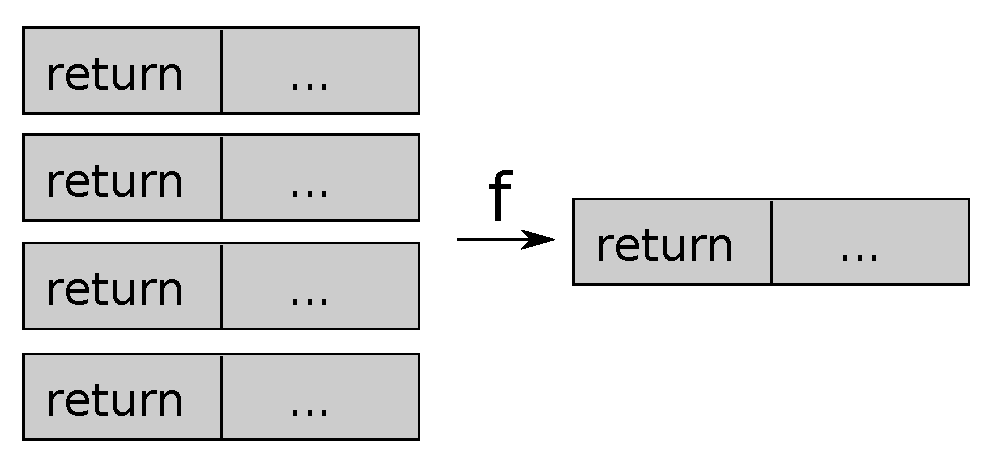
\includegraphics[height=100px]{purity-preservation}

Ist nicht sichergestellt, dass sämtliche Elemente der Eingabeliste rein sind, kann man sich weiter überlegen, dass eine
Möglichkeit zur Verfügung steht, mit der man den reinen Inhalt des monadischen Werts extrahieren kann - ähnlich wie
die unsichere Funktion \texttt{unsafePerformIO}, die den reinen Wert aus einer IO-Monade extrahiert, nur eben für
andere Monaden und sicher.
Es ist ja vorstellbar, dass man nur am reinen Ergebnis einer Funktion $f$ interessiert ist, unabhängig von eventuellen anhaftenden
monadischen Effekten. Tatsächlich kann man unter bestimmten Voraussetzungen zeigen, dass man beliebige Effekte in der 
Eingabeliste ignorieren kann, wenn man nur am reinen Ergebnis interessiert ist.

Sei $f :: Monad\ m \Rightarrow [m\ Int] \rightarrow m\ Int$, sei $\kappa$ eine Monadeninstanz und sei $p :: \kappa\ a \rightarrow a$, d.h. $p$ ist die erwähnte Funktion, die den reinen Wert aus dem monadischen Kontext extrahiert.
Wenn folgende Aussagen gelten:

\begin{itemize}
\item $p \circ return_{\kappa} = id$
\item Für beliebige Typen $t, t'$ und beliebige $m :: k\ t, k :: t \rightarrow k t'$ gilt\\
$p (m\ {>>=}_{\kappa}\ k) = p\ (k\ (p\ m))$
\end{itemize}

dann liefert $p \circ f_{\kappa}$ das gleiche Eregbnis für beliebige Listen gleicher Länge, deren Elemente an jeweils gleicher Position
die gleichen p-Bilder haben, sprich: den gleichen reinen Anteil. Man kann $p \circ f_{\kappa}$ kann also auch erhalten durch
$g \circ (map\ p)$ für eine passende Funktion $g :: [Int] \rightarrow Int$ \cite{voigtlander}.

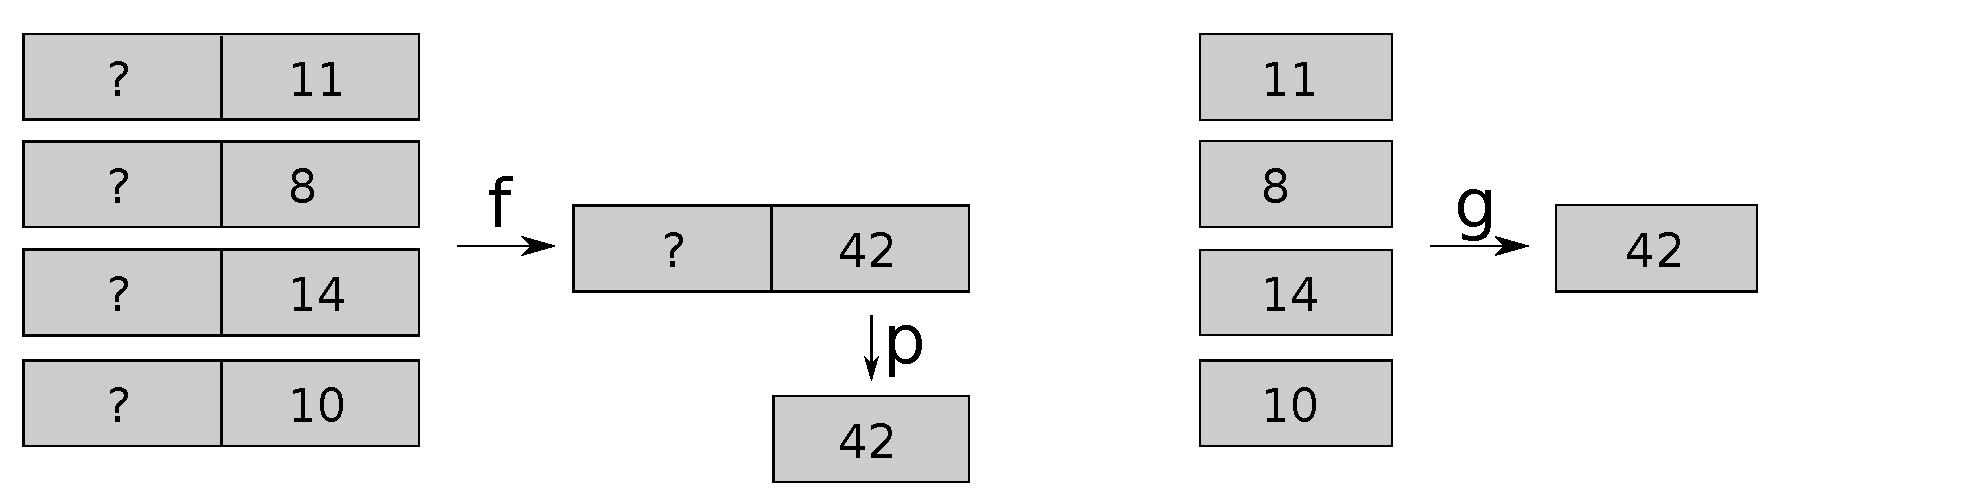
\includegraphics[height=100px]{safe-value-extraction}

Für diese Aussage werden keine Monadengesetze benötigt.